%%%%%%%%%%%%%%%%%%%%%%%%%%%%%%%%%%%%%%%%%%%%%%%%%%%%%%%%%%%%%%%%%%%%%%%%%%%%%%%%%%%%%%%%%%%%%%%%%%%%%%%%%%
%%%   %%%%
%%%%%%%%%%%%%%%%%%%%%%%%%%%%%%%%%%%%%%%%%%%%%%%%%%%%%%%%%%%%%%%%%%%%%%%%%%%%%%%%%%%%%%%%%%%%%%%%%%%%%%%%%%%

\documentclass[runningheads,a4paper]{llncs}

\usepackage[utf8]{inputenc}
\usepackage{amssymb}
\setcounter{tocdepth}{3}
\usepackage{graphicx}
\usepackage{tabularx}
\usepackage{url}
\usepackage{listings}
\usepackage{subfigure}
\usepackage{algorithmic}
\usepackage{algorithm}
\usepackage{verbatim}
\usepackage{subfig}
%\usepackage{lofdepth}

%\newcommand{\keywords}[1]{\par\addvspace\baselineskip
%\noindent\keywordname\enspace\ignorespaces#1}

% todo macro
\usepackage{color}
\newtheorem{deflda}{Axiom}
\newcommand{\todo}[1]{\noindent\textcolor{red}{{\bf \{TODO}: #1{\bf \}}}}
\newcommand{\neon}{NeOn }
\newcommand{\protege}{Prot{\'e}g{\'e} }



%%%%%%%%%%%%%%%%%%%%%%%%%%%%%%%
%%%  Beginning of document  %%%
%%%%%%%%%%%%%%%%%%%%%%%%%%%%%%%

\begin{document}


\title{QA4LOV: A Natural Language Interface to Linked Open Vocabulary}

\author{ Ghislain Auguste Atemezing\inst{1}, Pierre-Yves Vandenbussche\inst{2} }

\institute{
MONDECA, 35 Boulevard de Strasbourg, Paris, France. \\
\and Fujitsu, Galway, Ireland.\\
\email{ghislain.atemezing@mondeca.com} \\
\email{pierre-yves.vandenbussche@ie.fujitsu.com} \\
}

\maketitle


%%%%%%%%%%%%%%%%%%
%%%  Abstract  %%%
%%%%%%%%%%%%%%%%%%

\begin{abstract}

There is an increasing presence of structured data due to the adoption of Linked data principles on the web. At the same time, web users have different skills and want to be able to interact with Linked datasets in various manner, such as asking questions in natural language. 
%Over the last years, the QALD challenges series are becoming the references for benchmarking question answering systems. However, QALD questions are targeted on datasets, not on vocabulary catalogues. 
This paper proposed a first implementation of Query Answering system (QA) applied to the Linked Open Vocabularies (LOV) catalogue, mainly focused on metadata information retrieval. The goal is to provide to end users yet another access to metadata information available in LOV  using natural language questions.
% Currently, the system handles almost 92,99\% of the vocabularies in LOV.


\end{abstract}

\keywords{Question Answering, Vocabulary Catalogue, data usage, user experience}


%%%%%%%%%%%%%%%%%%%%%%%%%
%%%  1. Introduction  %%%
%%%%%%%%%%%%%%%%%%%%%%%%%

\section{Introduction}\label{sec:introduction}
The recent years have seen the adoption of semantic web in many domains, generating a mass of structured data available in RDF. Linked data has contributed to interlink different datasets across domains, where publishers use best practices for producing interoperable datasets by reusing ontologies and making alignments. 

However, users need to have a minimal knowledge of SPARQL language and RDF skills to query  RDF datasets. It is one barrier that is overcome by Question Answering (QA) systems, which directly take as input questions in natural language. The need for more advanced tools and QA systems that operate over large repositories of Linked Data has also been the motivation for the QALD Question Answering over Linked Data (QALD) series of workshops \cite{lopezetal2013}. 
%Started in 2011, QALD challenges offer a test sets questions whose answers can be found in the DBpedia and MusicBrainz, with more complex questions added each year. However, there is not yet a specific set of questions specific to retrieve metadata at schema level.
 
Vocabulary catalogues and semantic search engines are special datasets as classes and properties are used to model and generate datasets available in the Linked Data space. Ontologies are an important part in the semantic web layer to build full interoperable datasets. Most vocabulary catalogues provide terms search and APIs to access their datasets. LOV provides five types of search methods: metadata search, ontology search, APIs access, dump file in RDF and SPARQL endpoint access \cite{vandenbusschelov}.


This paper presents a prototype for a vocabulary backed question answering system that can transform natural language questions into SPARQL queries, thus giving the end users access to the information stored in vocabulary repositories. The paper is structured as follows: Section \ref{sec:questions} describes the system, followed by the set of questions in Section \ref{sec:system}. An evaluation is presented in Section \ref{sec:evaluation} and a short conclusion and future work in Section \ref{sec:conclusion}.  


%Consider the following question in natural language \textit{``What is dcterms?''}. The answer in English corresponds to the following SPARQL query in the LOV endpoint:\footnote{\url{http://lov.okfn.org/dataset/lov/sparql}}

%\begin{verbatim}
%PREFIX vann:<http://purl.org/vocab/vann/>
%PREFIX voaf:<http://purl.org/vocommons/voaf#>
%PREFIX dcterms: <http://purl.org/dc/terms/>

%SELECT DISTINCT ?x1  {
% 	GRAPH <http://lov.okfn.org/dataset/lov>{
% 	 	?x0 a voaf:Vocabulary.
%  ?x0 vann:preferredNamespacePrefix "dcterms".
%  ?x0 dcterms:description ?x1.
 	 
%}}
%\end{verbatim}

%%%%%%%%%%%%%%%%%%%%%%%%%%%%%%%
%%%  2. System Description  %%%
%%%%%%%%%%%%%%%%%%%%%%%%%%%%%%%

\section{System Description}
\label{sec:system}

The system receives as input a natural language question formulated in English and outputs the query that will retrieve the answer to the question from the LOV catalogue. The architecture of the system is illustrated in Fig.\ref{fig:q4lovarchi} and a screenshot of the live demo in Fig. \ref{fig:qa-screenshot}. The system is available at \url{http://lov.okfn.org/dataset/lov/qa}.

\begin{figure}
\centering
\begin{subfigure}
  \centering
  \includegraphics[width=.4\linewidth]{img/qa4lov-archi.pdf}
  \caption{System architecture}
  \label{fig:q4lovarchi}
\end{subfigure}%
\begin{subfigure}
  \centering
  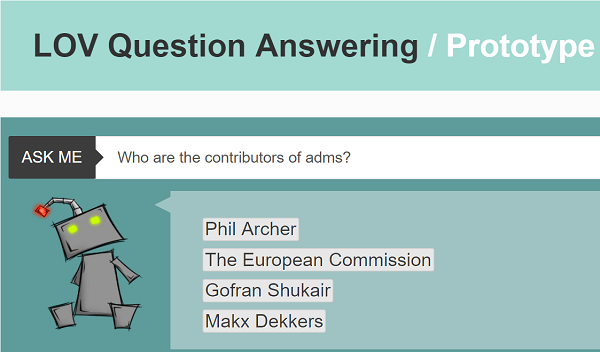
\includegraphics[width=.5\linewidth]{img/qa-screenshot.png}
  \caption{A screenshot showing the system answering to the contributors of adms}
  \label{fig:qa-screenshot}
\end{subfigure}
%\caption{A figure with two subfigures}
\label{fig:test}
\end{figure}



%\begin{figure}[ht!b]
%\centering
%\caption{Architecture of the system.}
%\includegraphics[scale=.6]{qa4lov-archi.pdf}
%\label{fig:q4lovarchi}
%\end{figure}
\todo{make this figure way shorter and add a screenshot}

The implementation uses the Quepy tool from Machinalis \footnote{\url{https://github.com/machinalis/quepy/}}. The POS tagset used by Quepy is the Penn Tagset \cite{marcus1993building}. First, regular expressions are defined to match the natural language questions and transform them into an abstract semantic representation. Then, specific templates are defined for the system to handle users' questions. To handle regular expressions, Quepy uses the \texttt{refo} library\footnote{\url{https://github.com/machinalis/refo}} which work with regular expressions as objects. 

A vocabulary is defined by a fixed relation \texttt{voaf:Vocabulary}\footnote{All the prefixes are the ones used at \url{http://lov.okfn.org/dataset/lov/vocabs}} and a POS associated to a \texttt{vann:preferredNamespacePrefix}. LOV uses a unique prefix to identify namespaces, which is a string from length 2 to length 17, although the recommendation for publishers is to use a prefix with less than 10 characters.
%\cite{pybernard12}.  

The syntactic processor is based on regular expressions using POS terms. As a vocabulary is identified by its prefix, we use  the following syntactic patterns: NN, NNS, FW, DT, JJ and VBN. Each question from Q1 to Q14 is associated to a unique template. After, when a prefix is recognized, the semantic interpreter uses fixed relations with the English tag, which are properties in RDF triple pattern. The code below show a regex for the contributors of a vocabulary 
\begin{verbatim}
regex1 = Pos("WP") + Lemma("be") + Pos("DT") + Lemma("contributor") + \
        Pos("IN") + Vocabulary()
\end{verbatim}

%\todo{provide an example of regex?}
%Table \ref{tab:propTable} presents the different fixed relations currently used in the system to cover the set of the 14 questions.

%\begin{table}
%\centering
%\caption{Relationship between Questions and Properties used to generate the SPARQL query from natural language}
%\label{tab:propTable}
%\begin{tabular}{|c|l|} \hline
%\textbf{Question ID} & \textbf{Property} \\ \hline
%\texttt{Q1} & \texttt{dcterms:description}  \\ \hline
%\texttt{Q2} & \texttt{dcterms:publisher}  \\ \hline 
%\texttt{Q3} & \texttt{dcterms:issued}  \\ \hline
%\texttt{Q4} & \texttt{dcterms:issued}  \\ \hline
%\texttt{Q5} & \texttt{dcterms:contributor}  \\ \hline
%\texttt{Q6} & \texttt{dcterms:modified}  \\ \hline
%\texttt{Q7} & \texttt{dcat:distribution}  \\ \hline
%\texttt{Q8} & \texttt{dcterms:language}  \\ \hline
%\texttt{Q9} & \texttt{foaf:homepage}  \\ \hline
%\texttt{Q10} & \texttt{voaf:reusedByVocabularies} \\ \hline
%\texttt{Q11} & \texttt{voaf:reusedByDatasets} \\ \hline
%\texttt{Q12} & \texttt{vann:preferredNamespaceUri} \\ \hline
%\texttt{Q13} & \texttt{dcterms:title} \\ \hline
%\texttt{Q14} & \texttt{dcat:keyword} \\ \hline

%\end{tabular}
%\end{table}





%%%%%%%%%%%%%%%%%%%%%%%%%%%%%%%
%%%  3. Questions  %%%
%%%%%%%%%%%%%%%%%%%%%%%%%%%%%%%
\section{Types of Questions}
\label{sec:questions}

LOV is a highly curated observatory of the semantic vocabularies ecosystem, with the aim of promoting the reuse of well-documented vocabularies in the Linked Data space. Each version of a vocabulary in LOV contains relevant metadata information which can be discovered by agents. 
%\begin{itemize}
%\item A preferred namespace, useful when the vocabulary is not dereference-able; 
%\item A URI, unique identifier of the vocabulary;
%\item A title, a short text; 
%\item A homepage, mainly a page where to find the documentation of the vocabulary;
%\item A description, which gives more information about the scope of the vocabulary;
%\item The creators of the vocabulary, represented by their URIs.
%\item The publishers of the vocabulary, and
%\item The different languages in which the vocabulary is available.
%\end{itemize}

Additionally, users could be interested in other interesting facts, such as the number of versions, the number of datasets  using the vocabulary, the number of external vocabularies reusing the vocabulary and the category to which belong the vocabulary. A first set of 14 questions in natural language can be handle by the prototype, covering different type of metadata information available in a vocabulary. Table \ref{tab:qtable} shows the list of questions, where in the column ``Template'', [be] can be either the present or the past form of the verb, and [vocab] is the preferred prefix of the vocabulary. The regex uses lemmas to combine different types of the questions accordingly.
%\todo{Here we have the feeling only be and vocab can change whereas in reality we use lemma or other words...}    

\begin{table*}
\centering
\caption{Questions in natural language for retrieving metadata information in a vocabulary catalog. }
\label{tab:qtable}
\begin{tabular}{|c|l|l|} \hline
\textbf{ID} & \textbf{Template} & \textbf{Sample Question}\\ \hline
\texttt{Q1} & \textit{What [be] [vocab]?} &  \textit{What is prov?} \\ \hline
\texttt{Q2} & \textit{Where [be] [vocab] from?} &  \textit{Where is foaf from?} \\ \hline
\texttt{Q3} & \textit{How old [be] [vocab]?} &  \textit{How old is prov?} \\ \hline
\texttt{Q4} & \textit{When [be] [vocab] release?} &  \textit{When was voaf release?} \\ \hline
\texttt{Q5} & \textit{Who [be] the contributors of [vocab]?} &  \textit{Who are the contributors of adms?} \\ \hline
\texttt{Q6} & \textit{When [be] [vocab] last update?} &  \textit{When was schema last update?} \\ \hline
\texttt{Q7} & \textit{What [be] the versions of [vocab]?} &  \textit{What are the versions of adms?} \\ \hline
\texttt{Q8} & \textit{What [be] the languages of [vocab]?} &  \textit{What are the languages of dcat?} \\ \hline
\texttt{Q9} & \textit{Where to find [vocab] documentation?} &  \textit{Where to find foaf documentation?} \\ \hline
\texttt{Q10} & \textit{How many vocabularies reuse [vocab]?} &  \textit{How many vocabularies reuse adms?} \\ \hline
\texttt{Q11} & \textit{How many datasets use [vocab]?} &  \textit{How many datasets use adms?} \\ \hline
\texttt{Q12} & \textit{What [be] the namespace of [vocab]?} &  \textit{What is the namespace of  dcterms?} \\ \hline
\texttt{Q13} & \textit{What [be] the title of [vocab]?} &  \textit{What is the title of foaf?} \\ \hline
\texttt{Q14} & \textit{What [be] the category of [vocab]?} &  \textit{What is the category of dcterms?} \\ \hline
\end{tabular}
\end{table*}



%%%%%%%%%%%%%%%%%%%%%%%%%%%%%
%%%  4.System evaluation  %%%
%%%%%%%%%%%%%%%%%%%%%%%%%%%%%

\section{System Evaluation}
\label{sec:evaluation}

%This first set of questions are not found in the QALD challenges, where answers had to be found either in DBpedia or in a federated dataset such as Yago2 and MusicBrainz. In terms of complexity, the test questions are either simple questions related to retrieve metadata information. 
The system allows users to interact with the LOV catalogue through the answers generated. Depending on the types of the results (e.g., agents, versions, categories), the system allows users to further explore the dataset with more interactions.
All the questions which generated SPARQL query gives satisfactory results. The most challenging issue is to determine the most suitable POS that cover all the vocabulary prefixes. For example, out of 528\footnote{This number corresponds to the total number of vocabularies inserted in LOV as of January, 8th 2016.} vocabularies in LOV, 13 of them contain an hyphen and the system can not generate query (e.g., \texttt{elseweb-modelling}). Moreover, 21 prefixes contain a number (e.g., \texttt{g50k}) and 3 special cases (\texttt{homeActivity}, \texttt{LiMo}, and \texttt{juso.kr})and are not currently covered by the system. Currently, the system handles 92,99\% of the prefixes in LOV.

%One of the issue dealing with QA over a vocabulary catalogue is to find relevant questions that can be asked against the system, based on the prefix. Since there is not a uniform way of describing a prefix, it is almost challenging to find the suitable pattern with NLP tools.  

%\todo{Find insights into specific challenges when doing QA over LOV}\\
%\todo{Find problems, if different, from the ones posed by e.g., querying DBpedia}\\
%\todo{complete type of questions covered}\\


%%%%%%%%%%%%%%%%%%%%%%%%%
%%%  4. Related work  %%%
%%%%%%%%%%%%%%%%%%%%%%%%%

%\section{Related Work}\label{sec:soa}


%%%%%%%%%%%%%%%%%%%%%%%%%%%%%%%%%%%%%%%
%%%  5. Conclusion and Future Work  %%%
%%%%%%%%%%%%%%%%%%%%%%%%%%%%%%%%%%%%%%%

\section{Conclusion and Future Work}
\label{sec:conclusion}
%\input{conclusion}

In this paper, we have presented a prototype system for answering a set of questions in natural language backed by a vocabulary catalogue. The questions are targeted to retrieve metadata information in vocabularies. Accessing LOV dataset by this system will hugely help lay users without SPARQL skills to interact more with the catalogue, and improve also the quality of the metadata by ontology publishers.  
%\todo{may be emphasize on the impact for end users...}
The implementation uses the LOV dataset in RDF and the Quepy tool. The first results show that the system handles 92,99\% of the metadata of vocabularies in the LOV catalogue.
We plan to extend the types of queries to more complex ones. Moreover, we can use various semantic relationships in LOV to do query expansion by using for instance sub-properties. 
%Also, we intend to align the set of questions to the QALD challenges to make the system comparable to existing Question Answering systems.  

%The approach is based on the identification of the vocabulary prefix combining POS and regular expressions.

%%%%%%%%%%%%%%%%%%%%%%%%%
%%%  Acknowledgments  %%%
%%%%%%%%%%%%%%%%%%%%%%%%%
%\vspace{1mm}
%\paragraph{\textbf{Acknowledgments}} %\label{sec:acknowledgments}
%Thanks to the LOV team and curators for maintaining the LOV catalogue, and Machinalis for the open source Quepy tool. 


\bibliographystyle{abbrv}
%\nocite{*}
\bibliography{qa4lov}
%\balancecolumns
\end{document}
